\setchapterpreamble[u]{\margintoc}
\chapter{Zero knowledge}
\labch{chapter13}


Abbiamo ora tutti gli strumento per studiare la zero knowledge, ovvero l'idea di trasmettere un segreto senza conoscere il segreto. Abbiamo due agenti Peggy e Victor, che sono rispettivamente \textbf{Proover} e \textbf{Verifier}. La situazione che vogliamo creare è la seguente: il proover conosce un segreto e vuole convincere il verifier che conosce il segreto, senza però comunicarlo al verifier; inoltre non vuole nemmeno che il verifier possa a dire ad altri che egli conosce il segreto.

Vogliamo quindi che il verifier apprenda solo la conoscenza che il proover conosce il segreto, ma senza che questa conoscenza sia sufficiente a convincere altri che il proover conosce il segreto. 
\\

\noindent \underline{Esempio}
\\
\begin{figure}
    \centering
    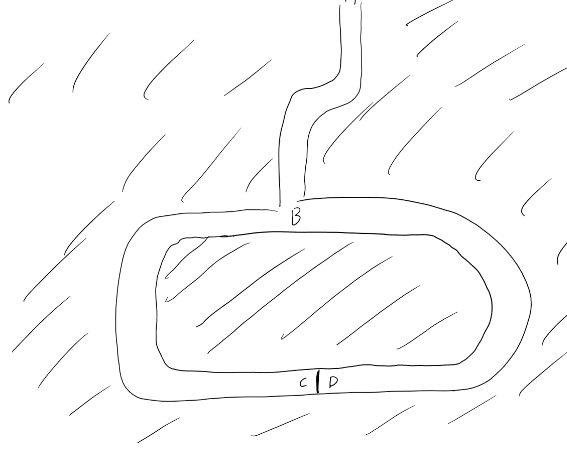
\includegraphics[width=0.8\textwidth]{images/13-1.png}
    \caption{Caverna}
    \label{fig:13-1}
\end{figure}

\noindent Supponiamo che $P$ e $V$ si trovino in una caverna come in figura \ref{fig:13-1}, dove le sezioni C e D sono separate da una porta che si apre solo con una parola chiave. $P$ vuole dimostrare a $V$ di conoscere la parola chiave. Vediamo come potrebbe fare:
\begin{itemize}
    \item $V$ segue $P$ mentre parte dal punto B e ritorna al punto B. IN questo modo però $V$ entra a conoscenza della parola segreta che apre al porta;
    \item $V$ aspetta $P$ al punto B e lo vede andare verso il lato C e tornare dal lato D. $V$ però potrebbe attaccare una videocamera a $P$ e mostrare il filmato ad altri per dimostrare che $P$ conosce la parola chiave.
\end{itemize}

\noindent Nessuna di queste due soluzione va bene. Proviamo a vederne una che applica il seguente protocollo:
\begin{enumerate}
    \item P, $V$ si trovano all'entrata della caverna (punto A);
    \item $P$ raggiunge B e lancia una moneta per decidere C o D;
    \item $P$ raggiunge C o D;
    \item $V$ raggiunge B e lancia una moneta per decidere C o D;
    \item $V$ chiede a $P$ di uscire dal lato risultante;
    \item $P$ obbedisce.
\end{enumerate}

\noindent Con questo protocollo se $P$ conosce il segreto non ha problemi, mentre se non lo conosce ha una probabilità di $\frac{1}{2}$ di essere scoperto da V, in quanto non sarebbe in grado di uscire dal lato richiesto. Di conseguenza $V$ ha una probabilità di $\frac{1}{2}$ di verificare correttamente se $P$ conosce o meno il segreto.

La probabilità che $V$ ha di sbagliare è troppo altra, dobbiamo fare in modo che si abbassi. Come possiamo fare? Possiamo ripetere il protocollo $k$ volte, rendendo la probabilità di sbagliare a $\frac{1}{2^k}$.
\\

\noindent Abbiamo quindi creato un protocollo dove:
\begin{itemize}
    \item Se $P$ conosce il segreto, allora $V$ lo accetterà sempre;
    \item Se $P$ non conosce il segreto, possiamo rendere la probabilità che $V$ accetti esponenzialmente piccola (sostanzialmente $V$ rifiuta). 
\end{itemize}

\noindent Questo protocollo risolve anche il problema del "filmato": poiché non viene filmata l'apertura della porta, potrebbe essere che $P$ e $V$ si fossero messi d'accordo prima di girare il filmato per convincere gli altri che $P$ conosca il segreto.

Abbiamo raggiunto la zero knowledge totale.

\section{Interactive Proof System per un linguaggio L}
Un IPS per un linguaggio L si compone di una coppia di algoritmi/macchine di Turing) $(P, V)$ tali che:
\begin{itemize}
    \item Il proover ha capacità di calcolo illimitata;
    \item Il verifier ha capacità di calcolo $\in PPT$.
\end{itemize}

\noindent Poiché dimostrare è più difficile dimostrare che verificare, al proover diamo una potenza di calcolo illimitata. $P$ e $V$ interagiscono scambiandosi messaggi. Alla fine $V$ accetta o rifiuta. 
\\

\noindent Un linguaggio $L$ ammette IPS se esistano $P, V$ tali che:
\begin{align*}
    &\forall x \in L \ Pr[(P, V) \text{ accetta } x] > \frac{2}{3}\\
    &\forall x \not\in L \ \forall P' \ Pr[(P', V) \text{ accetta } x] < \frac{1}{3}
\end{align*}

\noindent Nel primo caso va bene qualsiasi numero maggiore di $\frac{2}{3}$ (alta), mentre nel secondo minore di $\frac{1}{2}$ (bassa).

Qualunque linguaggio NP accetta un IPS. La classe dei linguaggi che ammette un IPS si chiama IP.

\subsection{Problema del Quadratic Non Residuosity}
Abbiamo un numero in $Z_n^*$ che non è un quadrato e vogliamo costruire un IPS che lo dimostri:
\begin{itemize}
    \item Input $(x, n)$;
    \item Output accetta se $x$ non è un quadrato.
\end{itemize}

\noindent Vediamo lo scambio di messaggi:
\begin{itemize}
    \item $V$ sceglie $w_1 \ ... \ w_n \in_R Z_n^*$, $b_1 \ ... \ b_n \in_R \{0, 1\}$ e invia a P: 
    \begin{align*}
        y_i = 
        \begin{cases} 
            W_i^2& \mbox{se }b_i = 0 \\ 
            W_ix^2& \mbox{se } b_i = 1
        \end{cases} 
    \end{align*}
    \item $P$ invia a $V$ la sequenza $c_1 \ ... \ c_n$, dove:
    \begin{align*}
        \forall i \ c_i =
        \begin{cases} 
            0& \mbox{se } y_i \text{ quadrato} \\ 
            1& \mbox{altrimenti }
        \end{cases}
    \end{align*}
    \item $V$ accetta se e solo se $b_1 \ ... \ b_l = c_1 \ ... \ c_l$.
\end{itemize}

\noindent Questo è un IPS in quanto. Se $x$ veramente non è un quadrato allora i $w_i$ saranno quadrati quando $b_i = 0$ e non quadrati quando $b_i = 1$. $P$ verifica la quadraticità dei $w_i$ ed effettivamente sarà il caso che i $b_i = c_i$.

Se invece $x$ è un quadrato, ovvero non appartiene al nostro linguaggio, tutti i $w_i$ sono quadrato. In questo caso, che $P$ conosca sia in grado di provare o no, non è in grado di ricavare informazione circa i $b_i$. Visto che i $b_i$ sono stati scelti a caso, per ogni $i$ la probabilità che $c_i$ sia uguale al $b_i$ è $\frac{1}{2}$. Quindi la probabilità che sia uguale per tutti gli $i$ è $\frac{1}{2^n}$.

Ripetendo l'esperimento più volte, la probabilità che $V$ accetti nel secondo caso diventa arbitrariamente piccola. 
\\

\noindent $P$ vuole dimostrare a $V$ di sapere la fattorizzazione di $n$. Come fa a dimostrarlo? Dice "dammi un numero e io ti dico se è un quadrato o no". Se $P$ è in grado di dire la quadraticità di un numero, vuol dire che $P$ conosce quell'informazione trapdoor che permette di capire se è un quadrato o un non quadrato. Ad oggi l'informazione trapdoor che permette di capire questo è la fattorizzazione di $n$.

\subsection{Problema dei Grafi non isomorfi}
Vogliamo stabilire se dati due grafi questi sono non isomorfi:
\begin{itemize}
    \item Input $(G_1, G_2)$, conosciuti da P, V;
    \item Output accetta se $x$ non è un quadrato.
\end{itemize}

\begin{definition}
    Due gradi sono isomorfi se traslando i nodi del grafo A nel grafo B, gli archi che esistono nel grafo A esistono anche nel grafo B.
\end{definition}

\noindent Vediamo lo scambio dei messaggi:
\begin{itemize}
    \item $V$ sceglie $i \in_R \{1, 2\}$, calcola $G'$ permutazione di casuale di $G_i$ e invia $G'$ a P;
    \item $P$ risponde: 
    \begin{align*}
        \begin{cases} 
            0& \mbox{se } G' \simeq G_1 \\ 
            1& \mbox{se } G' \simeq G_2
        \end{cases}
    \end{align*}
    \item $V$ accetta se $P$ indovina.
\end{itemize}

\noindent Se $G_1 \not\simeq G_2$, allora $G'$ è isomorfo solo al grafo da cui si è calcolata la permutazione. $P$ quindi indovina (avendo potenza di calcolo illimitata) e $V$ accetta il risultato con probabilità $1$. La capacita di $P$ di indovinare è legata puramente alla sua capacità di calcolo, in quanto non conosciamo alcuna informazione trapdoor per gli isomorfismi tra grafi. 
    
Se $G_1 \simeq G_2$ (ovvero non appartiene al linguaggio), $G'$ è isomorfo ad entrambi, e di conseguenza non contiene alcuna informazione circa la scelta fatta da $V$. $P$ può solo sparare a caso, avendo probabilità $\frac{1}{2}$ di indovinare $G_i$. 

Come sempre, ripetendo l'esperimento più volte, la probabilità che $V$ accetti nel secondo caso diventa arbitrariamente piccola. 
\\

\noindent Vogliamo arrivare ad un punto dove $V$ non impara nulla di più del semplice fatto che due grafi sono non isomorfi. In questo contesto, in realtà, $V$ è in grado di imparare qualcosa. Non propriamente il $V$ descritto sopra, ma un $V$ che cerca di sfruttate $P$ per imparare qualcosa di più. 

In generale abbiamo un $V$ che pone delle domande e un $P$ che risponde a queste domande, ma potremmo anche avere un $V$ non tanto interessato a capire che due grafi sono non isomorfi, ma che cerca di capire se un dato grafo $G_2$ e isomorfo a un altro grafo $G_3$. Parte da un'istanza in cui si vuole vedere se $G_1 \simeq G_2$ e mentre comunica con $P$ gli invia, come grafo da verificare, $G_3$ al posto di $G'$. Se $P$ risponde fa sapere a $V$ se $G_2 \simeq G_3$.

In generale questo si verifica quando $V$ vuole risolvere un problema ma non ha abbastanza potenza di calcolo per poterlo fare. Quindi pone il problema a P.

Vogliamo che $V$ non possa imparare nulla.
\\



\section{Zero knowledge}
Se prendiamo $(P, V)$ che interagiscono, la loro interazione genera una sequenza di messaggi. La sequenza è casuale, in quanto $P$ e $V$ lanciano monete (sono entrambi algoritmi stocastici -fanno scelte casuali-). Per essere precisi, dalla loro interazione si produce una misura di probabilità su sequenza di messaggi $View(P, V, x, h)$. La $View$ dipende dal proover, dal verifier, dalla stringa su cui stiamo cercando di riconoscere il linguaggio e da una sequenza $h$ (\textbf{hint}). L'\textbf{hint} serve per catturare l'idea che il verifier non riesce a ricavare alcuna informazione dall'interazione al proover nemmeno quando c'è una terza parte che fa domande al verifier (dà dei suggerimenti).\sidenote{Questo $h$ cattura il caso in cui qualcuno passa al verifier un grafo $G_3$ chiedendogli se è isomorfo a $G_1$ o $G_2$.
Un verifier che riceve una stringa $x$ in input su cui fare la verifica e un qualche suggerimento $h$, interagisce con il proover e da questa interazione si costruisce una misura di probabilità su questa sequenza di messaggi, chiamata $View(p, x)$. Quando abbiamo un IPS, vogliamo che un verifier non apprenda nulla (da protocollo). Il verifier che stiamo usando ora è un verifier fasullo $V'$, che appare a $P$ come il vero verifier, che fa domanda atte a ottenere altri risultati ($h$) non sia in grado di imparare nulla.} 

La $View(P, V, x, h)$ è il risultato tra l'interazione tra proover e verifier\sidenote{Praticamente è il filmato che $V$ ha fatto.}. Quando possiamo dire che il verifier non apprende nulla se non il fatto che $x \in L$ dall'interazione con P? L'unica cosa che $V$ ha in mano quando ha interagito con $P$ è un elemento campionato da $View$. Di conseguenza qualcuno che vede questa roba campionata da $View$, oppure vede più interazione tra $V$ e P\sidenote{È possibile effettuare delle indagini statistiche fino ad una quantità polinomiale di interazioni.}, non dice nulla ad una terza parte se il verifier poteva campionare messaggi dalla stessa misura di probabilità senza interagire con Proover. 

Se il verifier fosse in grado di costruire messaggi con la stessa misura di probabilità di $View$, potremmo dire che il fatto di vedere l'interazione tra $P$ e $V$ non dà info aggiuntive.
\\

\begin{definition}[(Perfect) zero knowledge]
    Diciamo che $P, V$ è \textbf{zero knowledge} se $\forall V' \in PPT$ esiste un simulatore $M\ in PPT$ tale che: 
    \begin{align*}
        M(P, V', x, h) = View(P, V', x, h)
    \end{align*}
\end{definition}    

\noindent Quindi esiste un algoritmo $M \in PPT$ che da solo produce sequenze di messaggi che sono distribuite come $View$\sidenote{Senza interagire con Proover, siamo in grado di costruire sequenze di messaggi scambiati tra $P$ e $V'$ con la stessa identica provabilità di $View$.}. Poiché possiamo usare il simulatore $M$ per generare la sequenza di messaggi, nessuno garantisce che $View(P, V, x, h)$ derivi dall'interazione tra $P$ e V, e che non sia stato generato da V.
\\

\noindent Possiamo definire tre tipi di zero knowledge:
\begin{enumerate}
    \item \textbf{Perfect Zero Knowledge}: la differenza tra $ View(P, V', x, h)$ e $M(P, V', x, h)$ è $0$:
    \begin{align*}
        View(P, V', x, h) = M(P, V', x, h)
    \end{align*}
    \item \textbf{Statistical Zero Knowledge}: la differenza tra $ View(P, V', x, h)$ e $M(P, V', x, h)$ è più piccola di ogni polinomio:
    \begin{align*}
        \sum_\alpha \big| View(P, V', x, h)(\alpha) - M(P, V', x, h)(\alpha) \big| < k^{-c}
    \end{align*}
    Non è necessario che il simulatore produce esattamente la stessa identica misura di probabilità prodotta da $View$, ma basta che le due misure sia sufficientemente vicine che nessun test statistico polinomiale possa vedere la differenza\sidenote{Se noi campioniamo più volte $View$ ed $M$, il numero di campioni che dobbiamo fare per vedere una differenza deve essere almeno pari al reciproco della differenza di probabilità sulle due cose che sto campionando. Quello che ci sta dicendo la formula è che la \textbf{somma} delle differenze di probabilità su tutti gli oggetti che stanno nello spazio campione della misura $View$ e della misura $M$ deve essere più piccola di qualsiasi polinomio. DI conseguenza, la quantità di esperimenti da fare per vedere una differenza è più grande di qualsiasi polinomio.}.
    
    \item \textbf{Computational Zero Knowledge}: $ View(P, V', x, h)$ e $M(P, V', x, h)$ sono computazionalmente (polinomialmente) indistinguibili\sidenote{Anche se vediamo il filmato, e questo è diverso dalla vera interazione tra Proover e Verifier, non siamo capaci di vedere la differenza. Non li sappiamo distinguere.}. Siano $P_k^{D, V}$ la probabilità che $D$ restituisca $1$ campionando da $View$ e $P_k^{D, M}$ la probabilità che $D$ restituisca $1$ campionando da $M$, allora:
    \begin{align*}
        \forall D \in PPT \left|P_k^{D, V} - P_k^{D, M}\right| < k^{\omega(1)}
    \end{align*}
\end{enumerate}

\noindent Dal punto di vista pratico, chiedere la perfect o la computational è la stessa cosa. inoltre perfect implica statistical e statistical implica computational.

\subsection{Problema del Ciclo hamiltoniano}
Verificare se $G$ ammette ciclo hamiltoniano. 

\begin{definition}[Ciclo hamiltoniano]
    Un ciclo hamiltoniano se esiste un cammino che visita ogni nodo esattamente una volta che riporta al nodo di partenza. 
\end{definition}

\noindent L'input è un grafo $G$ di cui non conosciamo un ciclo hamiltoniano. Vediamo lo scambio dei messaggi:
\begin{itemize}
    \item $P$ permuta $G$ per ottenere $H$, codifica tutti i bit della matrice di adiacenza di $H$ con bit commitment. Sia $H'$ il risultato;
    \item $P$ invia $H'$ a $V$;
    \item $V$ lancia una moneta per decidere se chiedere a P:
    \begin{itemize}
        \item[A.] L'evidenza che $G \simeq H$;
        \item[B.] L'evidenza che $H$ ammette ciclo hamiltoniano.
    \end{itemize}
    \item $P$ obbedisce. Per dare evidenza:
    \begin{itemize}
        \item[A.] Nel primo caso rivela $H$ e l'isomorfismo tra $G$ ed $H$\sidenote{Se due grafi sono isomorfi, uno ammette ciclo hamiltoniano se e solo se anche l'altro lo ammette.};
        \item[B.] Nel secondo caso scopre solo i bit di $H$ che costituiscono un ciclo hamiltoniano\sidenote{Il Proover non va a scoprire l'intera matrice di adiacenza, ma scopre solo alcuni archi, che sono quelli che mostrano che esiste un ciclo hamiltoniano. Effettivamente in questo caso il Verifier ha l'evidenza che la matrice di adiacenza di $H$ contiene un ciclo hamiltoniano, ma non ha altra conoscenza sulla struttura di $H$.}.
    \end{itemize}
\end{itemize}

\noindent Supponiamo che $G$ ammetta ciclo hamiltoniano. Allora quando $V$ fa al domanda, $P$ è in grado di rispondere ad entrambe le domande\sidenote{Il Proover ha costruito l'isomorfismo tra $G$ e $H$, quindi conosce $H$, $G$, l'isomorfismo (è in grado di scoprire tutto) e conosce il ciclo hamiltoniano su $G$. Conoscendo un ciclo hamiltoniano su $G$, allora può applicare l'isomorfismo che ha costruito per costruire un ciclo hamiltoniano su $H$. A questo punto è un grado di scoprire i bit di $H'$ corretti per rivelare l'esistenza del ciclo}. Quando $G$ ammette ciclo hamiltoniano e $P$ lo conosce, effettivamente il Proover è in gradi di rispondere sempre alle domande di $V$.

Se $G$ non ammette ciclo hamiltoniano, o il Proover non lo conosce (in un contesto la potenza di calcolo illimitata di $P$ deriva da una conoscenza di un'informazione trapdoor), allora quando il Proover manda un grafo $H$ coperto dal bit commitment al Verifier, non è possibile che $H$ sia contemporaneamente isomorfo a $G$ e ammetta ciclo hamiltoniano: 
\begin{itemize}
    \item Se $H$ è isomorfo a a $G$, allora anche $H$ non ammette ciclo hamiltoniano. Di conseguenza il Proover sa rispondere solo alla domanda \textbf{A};
    \item Se $H$ ammette ciclo hamiltoniano, allora $H$ non può essere isomorfo a $G$. DI conseguenza il Proover sa rispondere solo alla domanda \textbf{B}.
\end{itemize}

\noindent Visto che il verifier sceglie la domanda casualmente, con probabilità $\frac{1}{2}$, il Proover sa rispondere. 
\\

\noindent Questo è uno dei casi in cui $P$ conosce un segreto e $V$ vuole verificare quel segreto. Lo vogliamo fare in maniera tale che $V$ non possa usare l'interazione con $P$ per convincere altri. 

Come costruiamo $M$? Scegliamo casualmente la domanda di $V$. Se:
    \begin{itemize}
        \item La domanda è la \textbf{A}, costruiamo $H'$ secondo il protocollo ($H'$, domanda, risposta);
        \item La domanda è \textbf{B}, costruiamo $H'$ bit commitment del grafo completo. Scegliamo una permutazione casuale dei nodi come ciclo ($H'$, domanda, risposta).
    \end{itemize}

\noindent La distribuzione delle domande è quella corretta (con probabilità $\frac{1}{2}$ chiediamo la domanda \textbf{A}, con $\frac{1}{2}$ la domanda \textbf{B}); la distribuzione delle risposte è quella corretta: nel caso \textbf{A} è quella dovuta alla permutazione casuale del grafo, nel caso \textbf{B} è una permutazione casuale dei nodi di $H'$.  
Se prendiamo un grafo che ammette un ciclo hamiltoniano e ne permutiamo a caso i suoi nodi, questo diventa effettivamente la permutazione casuale dei nodi di un gradi. Quindi ogni permutazione dei nodi ha la stessa identica probabilità di essere un ciclo hamiltoniano, nel protocollo originale. Quindi anche la misura di probabilità delle risposte è quella originale. 

La misura di probabilità di $H'$ è uguale all'originale nel caso della domanda \textbf{A}, ma non nella domanda \textbf{B}. Nel caso \textbf{B} è un bit commitment non di una permutazione del grafo originale, ma di una permutazione di un grafo completo. Il punto chiave: prendiamo un qualunque osservatore che vede i messaggi costruiti da $M$e un osservatore che vede i messaggi scambiati da $P$ e $V$. Se questo osservatore ha potenza di calcolo polinomiale riesce a vedere la differenza? Vede che le domande sono distribuite uniformemente (scelte casualmente) e le risposte sono costruite correttamente. Però vediamo che il primo messaggio mandato, $H'$, in alcuni casi è il bit commitment della permutazione del grafo originale, negli altri casi è il bit commitment di un grafo completo. Ma un osservatore riesce a vedere che la matrice di adiacenza di $H'$ è uguale a quella di un grafo completo? Qualunque osservatore con potenza di calcolo polinomiale nono riesce ad avere alcuna informazione circa i bit nascosti da bit commitment. Di conseguenza non riesce a vedere la differenza.

Non è vero che quello che ha prodotto $M$ è identico all'interazione tra $P$ e $V$. Ma è vero che qualunque algoritmo con capacità di calcolo polinomiale, messo davanti all'interazione costruita da $M$ o a quella reale, non riesce a vedere la differenza. Le due misure di probabilità sono polinomialmente indistinguibili (solito concetto di distinguisher). 
\\

\noindent Questa cosa è computational zero knowledge in quanto nel caso \textbf{B} inviamo qualcosa di diverso rispetto alla normale interazione tra $P$ e $V$, solo che è indistinguibile all'esterno in quanto protetta con bit commitment.